%===============================================================================
% LaTeX sjabloon voor de bachelorproef toegepaste informatica aan HOGENT
% Meer info op https://github.com/HoGentTIN/latex-hogent-report
%===============================================================================

\documentclass[dutch,dit,thesis]{hogentreport}

\usepackage{lipsum} % For blind text, can be removed after adding actual content

%% Pictures to include in the text can be put in the graphics/ folder
\graphicspath{{../graphics/}}

%% For source code highlighting, requires pygments to be installed
%% Compile with the -shell-escape flag!
%% \usepackage[chapter]{minted}
%% If you compile with the make_thesis.{bat,sh} script, use the following
%% import instead:
\usepackage[chapter,outputdir=../output]{minted}
\usemintedstyle{solarized-light}

%% Formatting for minted environments.
\setminted{%
    autogobble,
    frame=lines,
    breaklines,
    linenos,
    tabsize=4
}

%% Ensure the list of listings is in the table of contents
\renewcommand\listoflistingscaption{%
    \IfLanguageName{dutch}{Lijst van codefragmenten}{List of listings}
}
\renewcommand\listingscaption{%
    \IfLanguageName{dutch}{Codefragment}{Listing}
}
\renewcommand*\listoflistings{%
    \cleardoublepage\phantomsection\addcontentsline{toc}{chapter}{\listoflistingscaption}%
    \listof{listing}{\listoflistingscaption}%
}

% Other packages not already included can be imported here

%%---------- Document metadata -------------------------------------------------
% TODO: Replace this with your own information
\author{Ian Daelman}
\supervisor{Dhr. T. Aelbrecht}
\cosupervisor{Dhr. K. Mekers}
\title{Hulp voor de Helpdesk: Virtuele Assistenten als Ondersteuningstool.}
\academicyear{\advance\year by -1 \the\year--\advance\year by 1 \the\year}
\examperiod{1}
\degreesought{\IfLanguageName{dutch}{Professionele bachelor in de toegepaste informatica}{Bachelor of applied computer science}}
\partialthesis{false} %% To display 'in partial fulfilment'
%\institution{Internshipcompany BVBA.}

%% Add global exceptions to the hyphenation here
\hyphenation{back-slash}

%% The bibliography (style and settings are  found in hogentthesis.cls)
\addbibresource{bachproef.bib}            %% Bibliography file
\addbibresource{../voorstel/voorstel.bib} %% Bibliography research proposal
\defbibheading{bibempty}{}

%% Prevent empty pages for right-handed chapter starts in twoside mode
\renewcommand{\cleardoublepage}{\clearpage}

\renewcommand{\arraystretch}{1.2}

%% Content starts here.
\begin{document}

%---------- Front matter -------------------------------------------------------

\frontmatter

\hypersetup{pageanchor=false} %% Disable page numbering references
%% Render a Dutch outer title page if the main language is English
\IfLanguageName{english}{%
    %% If necessary, information can be changed here
    \degreesought{Professionele Bachelor toegepaste informatica}%
    \begin{otherlanguage}{dutch}%
       \maketitle%
    \end{otherlanguage}%
}{}

%% Generates title page content
\maketitle
\hypersetup{pageanchor=true}

%%=============================================================================
%% Voorwoord
%%=============================================================================

\chapter*{\IfLanguageName{dutch}{Woord vooraf}{Preface}}%
\label{ch:voorwoord}

%% TODO:
%% Het voorwoord is het enige deel van de bachelorproef waar je vanuit je
%% eigen standpunt (``ik-vorm'') mag schrijven. Je kan hier bv. motiveren
%% waarom jij het onderwerp wil bespreken.
%% Vergeet ook niet te bedanken wie je geholpen/gesteund/... heeft

% TODO verder uitwerken van het voorwoord dit is louter een kladversie
De wereld verandert in hoog tempo, ook op het gebied van kunstmatige intelligentie. Dit biedt talloze mogelijkheden om bestaande processen kritisch te evalueren en te onderzoeken waar efficiëntiewinsten te behalen zijn. Om die reden heb ik besloten nader te onderzoeken hoe generatieve AI kan worden ingezet om de processen binnen mijn huidige werkomgeving te verbeteren. In het bijzonder wilde ik nagaan hoe we de supporttaken, die momenteel door het developmentteam van MyMinfin worden uitgevoerd, kunnen vergemakkelijken met behulp van generatieve AI.

Tevens maak ik van deze gelegenheid gebruik om mijn promotor, meneer Aelbrecht, en mijn co-promotor, Koen Meker, hartelijk te bedanken voor hun vele steun en waardevolle hulp tijdens het opstellen van deze bachelorproef.
%%=============================================================================
%% Samenvatting
%%=============================================================================

% TODO: De "abstract" of samenvatting is een kernachtige (~ 1 blz. voor een
% thesis) synthese van het document.
%
% Een goede abstract biedt een kernachtig antwoord op volgende vragen:
%
% 1. Waarover gaat de bachelorproef?
% 2. Waarom heb je er over geschreven?
% 3. Hoe heb je het onderzoek uitgevoerd?
% 4. Wat waren de resultaten? Wat blijkt uit je onderzoek?
% 5. Wat betekenen je resultaten? Wat is de relevantie voor het werkveld?
%
% Daarom bestaat een abstract uit volgende componenten:
%
% - inleiding + kaderen thema
% - probleemstelling
% - (centrale) onderzoeksvraag
% - onderzoeksdoelstelling
% - methodologie
% - resultaten (beperk tot de belangrijkste, relevant voor de onderzoeksvraag)
% - conclusies, aanbevelingen, beperkingen
%
% LET OP! Een samenvatting is GEEN voorwoord!

%%---------- Samenvatting -----------------------------------------------------
% De samenvatting in de hoofdtaal van het document

\chapter*{\IfLanguageName{dutch}{Samenvatting}{Abstract}}

% TODO dit is de samenvatting van het voorstel het moet verder aangevuld worden wanneer het onderzoek verder staat
Dit proces kan echter veel tijd en middelen vergen, vooral binnen grote organisaties. Het is vaak een uitdaging
om snel en adequaat antwoorden te bieden op vragen van klanten, wat resulteert in een aanzienlijke investering
van resources. Tegelijkertijd verwachten klanten een snelle oplossing voor hun problemen. Het is daarom in het
belang van zowel de organisatie als de klant om vragen efficiënt te beantwoorden.
Deze bachelorproef onderzoekt de mogelijkheden voor het ontwikkelen van een virtuele assistent die supportmedewerkers
kan ondersteunen bij het vinden van relevante antwoorden. Door middel van interviews met betrokkenen
wordt een analyse gemaakt van het huidige proces, met als doel de pijnpunten in het verwerken van
supporttickets in kaart te brengen. Daarnaast worden via een grondige literatuurstudie de verschillende opties
voor het inzetten van een virtuele supportassistent onderzocht. Het einddoel is het ontwikkelen van een proof of
concept dat bijdraagt aan een efficiëntere verwerking van klantvragen en de ondersteuning van medewerkers
bij het oplossen van deze problemen.
Het verwachte resultaat van dit onderzoek omvat enerzijds een overzicht van de mogelijkheden van een virtuele
supportassistent, met aandacht voor wat praktisch haalbaar is en welke factoren daarbij een rol spelen. Anderzijds
wordt op basis van een concrete casus een toepassing ontwikkeld in de vorm van een proof of concept (PoC).
Er wordt verwacht dat dergelijke virtuele assistenten in veel gevallen een meerwaarde kunnen bieden, maar niet
voor alle bedrijven. Afhankelijk van de specifieke behoeften en de manier waarop een organisatie een virtuele
assistent wil inzetten, moet eerst grondig worden geanalyseerd of een dergelijke implementatie daadwerkelijk
waarde toevoegt. Pas na een dergelijke analyse kan overwogen worden om een virtuele supportassistent te
implementeren.


%---------- Inhoud, lijst figuren, ... -----------------------------------------

\tableofcontents

% In a list of figures, the complete caption will be included. To prevent this,
% ALWAYS add a short description in the caption!
%
%  \caption[short description]{elaborate description}
%
% If you do, only the short description will be used in the list of figures

\listoffigures

% If you included tables and/or source code listings, uncomment the appropriate
% lines.
\listoftables

\listoflistings

% Als je een lijst van afkortingen of termen wil toevoegen, dan hoort die
% hier thuis. Gebruik bijvoorbeeld de ``glossaries'' package.
% https://www.overleaf.com/learn/latex/Glossaries

%---------- Kern ---------------------------------------------------------------

\mainmatter{}

% De eerste hoofdstukken van een bachelorproef zijn meestal een inleiding op
% het onderwerp, literatuurstudie en verantwoording methodologie.
% Aarzel niet om een meer beschrijvende titel aan deze hoofdstukken te geven of
% om bijvoorbeeld de inleiding en/of stand van zaken over meerdere hoofdstukken
% te verspreiden!

%%=============================================================================
%% Inleiding
%%=============================================================================

\chapter{\IfLanguageName{dutch}{Inleiding}{Introduction}}%
\label{ch:inleiding}

De inleiding moet de lezer net genoeg informatie verschaffen om het onderwerp te begrijpen en in te zien waarom de onderzoeksvraag de moeite waard is om te onderzoeken. In de inleiding ga je literatuurverwijzingen beperken, zodat de tekst vlot leesbaar blijft. Je kan de inleiding verder onderverdelen in secties als dit de tekst verduidelijkt. Zaken die aan bod kunnen komen in de inleiding~\autocite{Pollefliet2011}:

\begin{itemize}
  \item context, achtergrond
  \item afbakenen van het onderwerp
  \item verantwoording van het onderwerp, methodologie
  \item probleemstelling
  \item onderzoeksdoelstelling
  \item onderzoeksvraag
  \item \ldots
\end{itemize}

\section{\IfLanguageName{dutch}{Probleemstelling}{Problem Statement}}%
\label{sec:probleemstelling}

Uit je probleemstelling moet duidelijk zijn dat je onderzoek een meerwaarde heeft voor een concrete doelgroep. De doelgroep moet goed gedefinieerd en afgelijnd zijn. Doelgroepen als ``bedrijven,'' ``KMO's'', systeembeheerders, enz.~zijn nog te vaag. Als je een lijstje kan maken van de personen/organisaties die een meerwaarde zullen vinden in deze bachelorproef (dit is eigenlijk je steekproefkader), dan is dat een indicatie dat de doelgroep goed gedefinieerd is. Dit kan een enkel bedrijf zijn of zelfs één persoon (je co-promotor/opdrachtgever).

\section{\IfLanguageName{dutch}{Onderzoeksvraag}{Research question}}%
\label{sec:onderzoeksvraag}

Wees zo concreet mogelijk bij het formuleren van je onderzoeksvraag. Een onderzoeksvraag is trouwens iets waar nog niemand op dit moment een antwoord heeft (voor zover je kan nagaan). Het opzoeken van bestaande informatie (bv. ``welke tools bestaan er voor deze toepassing?'') is dus geen onderzoeksvraag. Je kan de onderzoeksvraag verder specifiëren in deelvragen. Bv.~als je onderzoek gaat over performantiemetingen, dan 

\section{\IfLanguageName{dutch}{Onderzoeksdoelstelling}{Research objective}}%
\label{sec:onderzoeksdoelstelling}

Wat is het beoogde resultaat van je bachelorproef? Wat zijn de criteria voor succes? Beschrijf die zo concreet mogelijk. Gaat het bv.\ om een proof-of-concept, een prototype, een verslag met aanbevelingen, een vergelijkende studie, enz.

\section{\IfLanguageName{dutch}{Opzet van deze bachelorproef}{Structure of this bachelor thesis}}%
\label{sec:opzet-bachelorproef}

% Het is gebruikelijk aan het einde van de inleiding een overzicht te
% geven van de opbouw van de rest van de tekst. Deze sectie bevat al een aanzet
% die je kan aanvullen/aanpassen in functie van je eigen tekst.

De rest van deze bachelorproef is als volgt opgebouwd:

In Hoofdstuk~\ref{ch:stand-van-zaken} wordt een overzicht gegeven van de stand van zaken binnen het onderzoeksdomein, op basis van een literatuurstudie.

In Hoofdstuk~\ref{ch:methodologie} wordt de methodologie toegelicht en worden de gebruikte onderzoekstechnieken besproken om een antwoord te kunnen formuleren op de onderzoeksvragen.

% TODO: Vul hier aan voor je eigen hoofstukken, één of twee zinnen per hoofdstuk

In Hoofdstuk~\ref{ch:conclusie}, tenslotte, wordt de conclusie gegeven en een antwoord geformuleerd op de onderzoeksvragen. Daarbij wordt ook een aanzet gegeven voor toekomstig onderzoek binnen dit domein.
\chapter{\IfLanguageName{dutch}{Stand van zaken}{State of the art}}%
\label{ch:stand-van-zaken}

% Tip: Begin elk hoofdstuk met een paragraaf inleiding die beschrijft hoe
% dit hoofdstuk past binnen het geheel van de bachelorproef. Geef in het
% bijzonder aan wat de link is met het vorige en volgende hoofdstuk.

% Pas na deze inleidende paragraaf komt de eerste sectiehoofding.

\section{Inleiding}
In dit hoofdstuk wordt de werking van een Retrieval-Augmented Generation (RAG) model besproken. We behandelen de belangrijkste concepten en recente ontwikkelingen binnen zowel RAG als Large Language Models (LLM). Dit overzicht biedt inzicht in de huidige stand van zaken en vormt de basis voor een weloverwogen keuze bij de ontwikkeling van een Proof of Concept (PoC).

Concreet komen de volgende onderwerpen aan bod:
\begin{itemize}
    \item \textbf{Wat is RAG} – Wat is Retrieval-Augmented Generation en waarvoor is het geschikt?
    \item \textbf{De AI Act en de belangrijkste richtlijnen} – een overzicht van de relevante wet- en regelgeving en de impact hiervan op RAG-toepassingen.
    \item \textbf{Best practices voor IT-supportprocessen} – inzichten in hoe RAG kan worden toegepast binnen IT-support en welke methodologieën daarbij best worden gevolgd.
\end{itemize}

De nadruk zal voornamelijk liggen op het eerste luik, \textit{Wat is Retrieval-Augmented Generation (RAG) en waarvoor is het geschikt?}, aangezien dit een cruciale factor is voor het maken van een doordachte keuze bij de verdere uitwerking van de PoC. Indien nodig zullen de overige onderwerpen verder worden uitgediept.

\section{Wat is Retrieval-Augmented Generation en waarvoor is het geschikt?}
 
    \subsection{Introductie}   
    \textit{Large Language Models} (LLM) hebben de afgelopen jaren een enorme opmars gemaakt en vandaag de dag hebben deze modellen een brede impact op verschillende domeinen in de samenleving. Ondanks hun indrukwekkende mogelijkheden brengen LLM’s ook enkele nadelen met zich mee. Zo kunnen ze hallucineren, beschikken ze niet altijd over de meest actuele informatie, en missen ze vaak diepgaande domeinspecifieke kennis.  
    
    Een mogelijke oplossing voor deze beperkingen is \textit{Retrieval-Augmented Generation} (RAG). Deze techniek combineert de kracht van LLM’s met externe databronnen om nauwkeurigere en beter onderbouwde antwoorden te genereren. In deze sectie wordt toegelicht wat RAG is, hoe het werkt en op welke manier het kan bijdragen aan de ontwikkeling van een effectieve supportbot.
    
    \paragraph{Wat is RAG}
    RAG is, zoals eerder vermeld, een techniek die een antwoord biedt op de tekortkomingen van klassieke LLM’s. Door gebruik te maken van externe databronnen kunnen betere resultaten worden behaald dan met een traditionele LLM. Deze techniek maakt het mogelijk om domeinspecifieke data te integreren en de modellen bij te werken met actuele informatie. Hierdoor kunnen klassieke LLM’s verrijkt worden met nieuwe, up-to-date data die voldoet aan specifieke behoeften \autocite{Wu2024}.
    
    Om RAG in de praktijk toe te passen, moeten een aantal stappen worden doorlopen. Deze worden in het volgende deel nader toegelicht, maar samengevat bestaat het proces uit de volgende fasen:
    
    \begin{enumerate}
        \item \textbf{Indexeren}
        \item \textbf{Ophalen}
        \item \textbf{Verrijking}
        \item \textbf{Generatie}
    \end{enumerate}
    
    Deze stappen worden in het volgende deel uitgebreid besproken. Aan het einde van dit proces kan een gebruiker de functionaliteiten van een LLM koppelen aan de relevante documenten en gegevens die benodigd zijn.
    
    \subsection{Hoe werkt RAG}
    
    RAG kan worden samengevat in drie grote delen, het eerste deel is het ophalen van de info die van belang is (Retrieval). De tweede stap is het verrijken van het antwoord aan de hand van de documentatie die werd voorzien. Ten laatste blijft nog de generatie over. In deze stap wordt op basis van een LLM een antwoord gegeven aan de vraagstellen. Hieronder is een figuur te zien die dit illustreert.
    
     \begin{figure}[H]
        \centering
        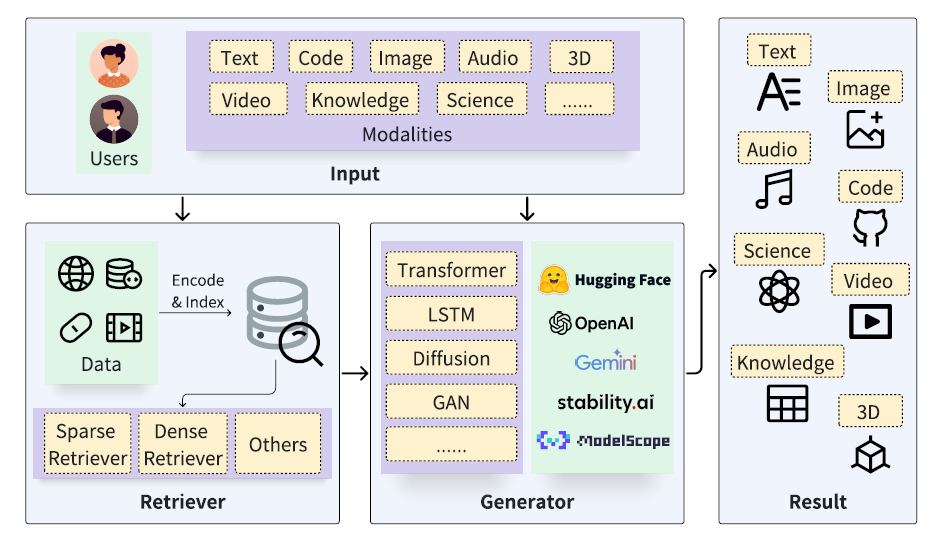
\includegraphics[width=\textwidth]{genericRAGArchitecture.png}
        \caption{Een generieke RAG architectuur \cite{Zhao2024}}
        \label{fig:livebench}
    \end{figure}
    
        \subsubsection{Ophalen}
            \paragraph{Indexeren}
        \subsubsection{Verrijken}
        \subsubsection{Generatie}
    
    
    \subsection{Bouwstenen van RAG}
    
    
        \subsubsection{LLM-modellen voor Retrieval-Augmented Generation (RAG)}
        Welke bestaande LLM-modellen kunnen worden gebruikt voor het ontwikkelen van een Retrieval-Augmented Generation (RAG)? 
        
        %TODO opzoeken wat LLM benchmarks zijn en hoe je ze in deze context kan gebruiken
        
        \paragraph{Introductie}
        Om te bepalen welke modellen het meest geschikt zijn voor de ontwikkeling van een RAG-model, is een objectieve meetmethode noodzakelijk. Gelukkig bestaan er verschillende platforms die LLM's vergelijken en rangschikken op basis van prestaties. In deze sectie bespreken we enkele van deze platforms en maken we een selectie van modellen die het meest geschikt lijken voor het bouwen van een RAG-model.
        
        %TODO overall dieper ingaan hoe ze te werk gaan als het gaat om vergelijken van een LLM dus de paper lezen en samenvatten wat je ermee kan gaan doen
        
        \paragraph{LiveBench} 
        Een platform dat LLM-modellen evalueert, is LiveBench. Dit platform stelt een rangschikking op voor verschillende modellen en biedt een actuele leaderboard die elke zes maanden wordt bijgewerkt. Voor deze bachelorproef zal gebruik worden gemaakt van de ranking afkomstig uit november 2024.
        
        LiveBench beoordeelt LLM-modellen op basis van zes categorieën. Binnen elke categorie worden meerdere taken uitgevoerd om een nauwkeurige beoordeling te verkrijgen. De zes categorieën zijn:
        \begin{itemize}
            \item Wiskundige vaardigheden (Math)
            \item Programmeervaardigheden (Coding)
            \item Redeneren en probleemoplossing (Reasoning)
            \item Data-analyse (Data Analysis)
            \item Volgen van instructies (Instruction Following)
            \item Begrip van natuurlijke taal (Language Comprehension)
        \end{itemize}
        
        Elke categorie wordt geëvalueerd op basis van specifieke taken. Dit resulteert uiteindelijk in een algemene rangschikking, waarin zowel de beste modellen per categorie als het beste presterende model overall worden geïdentificeerd.
        
        \begin{figure}[H]
            \centering
            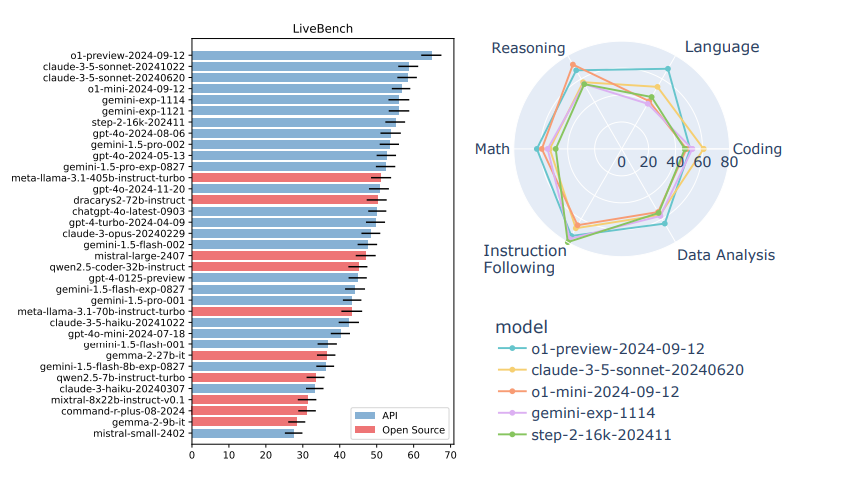
\includegraphics[width=\textwidth]{LiveBenchRanking.png}
            \caption{LiveBench ranking van verschillende LLMs.}
            \label{fig:livebench}
        \end{figure}
        
        \noindent\textbf{Bron:} \textit{LiveBench AI} \url{https://livebench.ai/#/details} (Geraadpleegd op 16 februari 2025).
        
        Uit de ranking van LiveBench kan geconcludeerd worden dat 3 verschillende organisaties elk een model aanbieden die vanuit globaal oogpunt tot de top 3 behoort. Deze top 3 zijn: 
        \begin{enumerate}
            \item claude-3-5-sonnet-20240620 van Anthropic
            \item Meta-llama-3.1-405b-instruct-turbo van Meta
            \item gpt-4o-2024-05-13 van OpenAI
        \end{enumerate}
        
        \subsubsection{Chatbot arena} 
        
        %TODO uitleggen hoe de scoring werkt van chatbot en eventueel uitleggen wat de verschillen zijn met LiveBench, ik denk vooral dat Chatbot arena getest wordt door mensen en zij hun mening op een grote schaal uitdrukken
        Een andere benchmark tool Chatbot arena, net zoals livebench is Chatbot arena een site die een actuele weergave biedt van de beste LLM's op basis van vooraf gedefinieerde catgeoriën. Op het moment van het schrijven van deze literatuurstudie is de top 3 LLM's volgens deze site de volgende:
        
        \begin{enumerate}
            \item GPT-4-Turbo van OpenAI
            \item GPT-4-0613 van OpenAI
            \item Mistral-Medium Mistral AI
        \end{enumerate}
        
        Hoewel het doel van beide benchmarks hetzelfde is is de manier van werken wel anders. ChatbotArena gaat gebruikers twee anonieme LLM modellen tegenover elkaar plaatsen, de gebruiker kan vervolgens een eigen vraag stellen en de gebruiker bepaalt zelf welke van de 2 het beste resultaat heeft opgeleverd.
        
        Het voordeel van deze methode is dat de LLM-modellen realistische cases moeten behandelen die door gebruikers zelf worden gesteld. Op basis van resultaten die de LLM modellen tonen kan een gebruiker zijn voorkeur meegeven. Het nadeel van deze manier van werken is dat de gebruikers die deze testen uitvoeren niet respresentatief zijn voor alle gebruikers van LLM-modellen. De gebruikers die deze testen uitvoeren zijn vaak mensen met een interesse in LLM-modellen of mensen die onderzoek doen in dit vakgebied. Desoondanks kan op basis van deze stemmen verscheidene modellen tegenover elkaar worden geplaatst. In januari 2024 werden ruim 240.000 stemmen uitgebracht door ongeveer 90.000 gebruikers \autocite{Chiang2024}. 
        
        %TODO Hier dit verder uitschrijven, ik denk niet dat je de volgende vraag kan beantwoorden dus ik zou meteen nagaan welke tools, frameworks er zijn die je kan gebruiken.
        
        %TODO zet hier ook de actuele ranking van beide benchmarks. Al was het maar om te duiden dat het een sterk veranderende wereld is waar en dat naar alle waarschijnlijkheid de modellen die nu worden gebruikt waarschijnlijk al achterhaald zullen zijn.
        
        \paragraph{Conclusie}
        Op basis van de 2 benchmarks die hier werden besproken kan niet meteen éénduidig besloten worden welke modellen het best zouden gebruikt worden voor het maken van het RAG model. Aangezien dit een zeer volatiele omgeving is met veel en snelle ontwikkelingen zijn de modellen die vandaag het beste scoren over een maand potentieel voorbij gestoken door nieuwe modellen. Desalniettemin bevatten deze benchmarks heel wat nuttige informatie en inzichten over de sterktes van bepaalde modellen tegenover andere modellen. 
     
    \subsection{RAG voor documentgebaseerde ondersteuning}
    Welke bestaande tools en frameworks kunnen bijdragen aan het opzetten van een RAG?
    
    \subsection{Tools en frameworks voor RAG}
    Welke bestaande tools en frameworks kunnen bijdragen aan het opzetten van een RAG?

\section{De AI Act en de belangrijkste richtlijnen}
Wat houdt de AI Act in, en wat zijn de belangrijkste richtlijnen die hierin moeten worden gevolgd?

\section{Best practices voor IT-supportprocessen}
Wat zijn de bestaande best practices voor de organisatie van IT-supportprocessen?

%%=============================================================================
%% Methodologie
%%=============================================================================

\chapter{\IfLanguageName{dutch}{Methodologie}{Methodology}}%
\label{ch:methodologie}

%% TODO: In dit hoofstuk geef je een korte toelichting over hoe je te werk bent
%% gegaan. Verdeel je onderzoek in grote fasen, en licht in elke fase toe wat
%% de doelstelling was, welke deliverables daar uit gekomen zijn, en welke
%% onderzoeksmethoden je daarbij toegepast hebt. Verantwoord waarom je
%% op deze manier te werk gegaan bent.
%% 
%% Voorbeelden van zulke fasen zijn: literatuurstudie, opstellen van een
%% requirements-analyse, opstellen long-list (bij vergelijkende studie),
%% selectie van geschikte tools (bij vergelijkende studie, "short-list"),
%% opzetten testopstelling/PoC, uitvoeren testen en verzamelen
%% van resultaten, analyse van resultaten, ...
%%
%% !!!!! LET OP !!!!!
%%
%% Het is uitdrukkelijk NIET de bedoeling dat je het grootste deel van de corpus
%% van je bachelorproef in dit hoofstuk verwerkt! Dit hoofdstuk is eerder een
%% kort overzicht van je plan van aanpak.
%%
%% Maak voor elke fase (behalve het literatuuronderzoek) een NIEUW HOOFDSTUK aan
%% en geef het een gepaste titel.


\section{Literatuurstudie}
Voor de opstart van deze bachelorproef is een uitgebreide literatuurstudie essentieel om de bestaande mogelijkheden op het gebied van virtuele assistenten te verkennen. Deze studie richt zich op een vergelijkende analyse die inzicht biedt in de verschillende beschikbare opties voor het ontwikkelen van een virtuele supportassistent. Hierbij worden de voor- en nadelen van elke optie in kaart gebracht, zodat op basis van deze informatie een onderbouwde keuze kan worden gemaakt voor de uitwerking van een PoC. De literatuurstudie moet ook duidelijkheid verschaffen over de benodigde hardware- en softwarevereisten voor de ontwikkeling.

Op basis van de literatuurstudie moet een analyse worden opgesteld om na te gaan welke optie die werden besproken binnen de literatuurstudie het best in overweging worden genomen. De belangrijkste keuze die zal moeten gemaakt worden binnen deze use case is de keuze tussen een RAG implementatie of een CAG implementatie. Aangezien beide voor- en nadelen hebben moet dit weloverwogen worden voor het opstellen van de PoC en het LLM modellen die kunnen worden gebruikt voor de PoC.


\section{Requirement analyse}


Gekoppeld aan de literatuurstudie zullen interviews worden afgenomen. Het doel van deze interviews is om een helder overzicht te verkrijgen van de verschillende vereisten voor de virtuele assistent. Op basis van het overzicht uit de literatuurstudie kan vervolgens een meer gerichte selectie worden gemaakt van de verschillende opties. Het uiteindelijke doel is om voor twee à drie modellen een PoC uit te werken die verder getest kunnen worden. Het is met andere woorden van belang om de verschillende modellen zo uitgebreid mogelijk te onderzoeken, zodat zoveel mogelijk modellen getoetst kunnen worden aan de gevraagde vereisten.Eens de literatuurstudie is afgerond en de interviews zijn afgenomen, kan met behulp van een MoSCoW-analyse een rangschikking worden opgesteld van de verschillende beschikbare modellen. Deze rangschikking bepaalt welke modellen worden geselecteerd voor het uitwerken van een PoC.

\section{Long list}

\section{Short list}

\section{Opstellen PoC}

\section{Uitvoeren testen en analyse resultaten}

Elk van de geselecteerde modellen wordt vervolgens uitgewerkt in een PoC. Zodra de verschillende PoC’s beschikbaar zijn, wordt een vergelijking gemaakt tussen de modellen. Hierbij worden de volgende aspecten specifiek getest:

\begin{itemize} 
    \item Wat is de kwaliteit van de antwoorden? 
    \item Wat is de tijd en de kost van een query?
    \item Hoe eenvoudig is het om het model op te zetten? 
\end{itemize}

De kwaliteit van de antwoorden zal worden gemeten aan de hand van de ROUGE-score, terwijl de tijd per query gemeten en vergeleken zal worden per model. Gezien het derde criterium eerder subjectief is, zal dit minder doorwegen in de uiteindelijke vergelijking. Aan de hand van deze drie criteria zal uiteindelijk een vergelijking worden gemaakt, waaruit zal blijken welk model het beste voldoet aan de gevraagde functionaliteit. Zo kan aan het einde van het onderzoek worden bepaald welke van de verschillende PoC's de meeste troeven heeft om in de praktijk te worden gebruikt.




% Voeg hier je eigen hoofdstukken toe die de ``corpus'' van je bachelorproef
% vormen. De structuur en titels hangen af van je eigen onderzoek. Je kan bv.
% elke fase in je onderzoek in een apart hoofdstuk bespreken.

%\input{...}
%\input{...}
%...

%%=============================================================================
%% Conclusie
%%=============================================================================

\chapter{Conclusie}%
\label{ch:conclusie}

% Trek een duidelijke conclusie, in de vorm van een antwoord op de
% onderzoeksvra(a)g(en). Wat was jouw bijdrage aan het onderzoeksdomein en
% hoe biedt dit meerwaarde aan het vakgebied/doelgroep? 
% Reflecteer kritisch over het resultaat. In Engelse teksten wordt deze sectie
% ``Discussion'' genoemd. Had je deze uitkomst verwacht? Zijn er zaken die nog
% niet duidelijk zijn?
% Heeft het onderzoek geleid tot nieuwe vragen die uitnodigen tot verder 
%onderzoek?


% onderzoeksvra(a)g(en). Wat was jouw bijdrage aan het onderzoeksdomein en
% hoe biedt dit meerwaarde aan het vakgebied/doelgroep? 
% Reflecteer kritisch over het resultaat. In Engelse teksten wordt deze sectie
Dit onderzoek biedt een helder overzicht van de verschillende mogelijkheden om een virtuele assistent te ontwikkelen. De uitgevoerde literatuurstudie maakt het mogelijk om, afhankelijk van de specifieke usecase, een weloverwogen keuze te maken tussen de verschillende benaderingen. Daarnaast werd een PoC uitgewerkt die aantoont hoe één van deze benaderingen,in dit geval RAG, kan worden toegepast in de praktijk. Niet alleen de PoC, maar ook de problemen die zich stelde tijdens de ontwikkeling bieden waardevolle lessen voor iedereen die een vergelijkbare PoC wil realiseren.
\\[1em]
De resultaten tonen aan dat de keuze van het LLM-model een cruciale rol speelt. Niet elk model is geschikt voor elke taak, zoals duidelijk werd bij functionaliteiten zoals tool calling. Binnen deze studie konden echter enkel kleinere modellen worden getest, waardoor niet uitgesloten kan worden dat krachtigere varianten van dezelfde modellen deze beperkingen ook hebben.
\\[1em]
Heel wat aspecten binnen dit onderzoek werden proefondervindelijk getest. De keuzes die binnen deze PoC gemaakt werden, zijn echter niet per definitie de beste voor elke RAG usecase. Elke toepassing vraagt om een specifieke afweging, afhankelijk van context, noden en technische randvoorwaarden.
\\[1em]
Het zou daarom waardevol zijn om in vervolgonderzoek niet enkel modellen onderling te vergelijken, maar ook andere aspecten van een RAG-architectuur nader te analyseren. Een eerste voorbeeld is het effect van verschillende parsers op ongestructureerde bestanden. Het is interessant om na te gaan welke parser het best omgaat met complexe PDF-bestanden die niet uitsluitend uit tekst bestaan, zoals gescande documenten of formulieren met tabellen en grafieken.
\\[1em]
Een tweede mogelijk onderzoekspiste betreft de impact van verschillende retrieval-methodes. Momenteel zijn er vier methodes beschikbaar, elk met een eigen aanpak voor het ophalen van documenten uit de vectordatabase. Een vergelijking van deze methodes op vlak van nauwkeurigheid, snelheid en robuustheid kan waardevolle inzichten opleveren.
\\[1em]
Een derde mogelijkheid is het analyseren van het effect van modelgrootte. In dit onderzoek werden voornamelijk modellen gebruikt met een vergelijkbaar aantal parameters. Het zou echter interessant zijn om na te gaan hoe verschillende versies van eenzelfde model met meer of minder parameters presteren in een RAG-context. Dit kan duidelijkheid scheppen over de verhouding tussen prestaties en efficiëntie.
\\[1em]
Tot slot kan het ook waardevol zijn om alternatieven voor RAG te verkennen. Binnen dit onderzoek werd bewust gekozen voor een RAG aanpak, maar gezien de snelle evolutie van LLM's en de steeds grotere context die deze modellen ter beschikking hebben kan het relevant zijn om te onderzoeken hoe een CAG systeem functioneert en of dit een valabel alternatief kan vormen.
\\[1em]
Samenvattend toont deze bachelorproef aan dat RAG een haalbare en veelbelovende aanpak is voor de ontwikkeling van een LLM-gebaseerde IT-supportbot in de context van MyMinfin. De opgedane inzichten vormen een stevige basis voor verdere optimalisatie en uitbreiding van dergelijke toepassing in de toekomst.

%---------- Bijlagen -----------------------------------------------------------

\appendix

\chapter{Onderzoeksvoorstel}

Het onderwerp van deze bachelorproef is gebaseerd op een onderzoeksvoorstel dat vooraf werd beoordeeld door de promotor. Dat voorstel is opgenomen in deze bijlage.

%% TODO: 
%\section*{Samenvatting}

% Kopieer en plak hier de samenvatting (abstract) van je onderzoeksvoorstel.

% Verwijzing naar het bestand met de inhoud van het onderzoeksvoorstel
%---------- Inleiding ---------------------------------------------------------

% TODO: Is dit voorstel gebaseerd op een paper van Research Methods die je
% vorig jaar hebt ingediend? Heb je daarbij eventueel samengewerkt met een
% andere student?
% Zo ja, haal dan de tekst hieronder uit commentaar en pas aan.

%\paragraph{Opmerking}

% Dit voorstel is gebaseerd op het onderzoeksvoorstel dat werd geschreven in het
% kader van het vak Research Methods dat ik (vorig/dit) academiejaar heb
% uitgewerkt (met medesturent VOORNAAM NAAM als mede-auteur).
% 

\section{Inleiding}%
\label{sec:inleiding}

Een ontwikkelingsteam heeft diverse verantwoordelijkheden. Naast hun primaire taak, het ontwikkelen van software, is het ook essentieel dat ze documentatie aanleveren. Dit kan variëren van API-documentatie voor andere teams tot een beginnersgids voor nieuwe medewerkers. Het is belangrijk dat deze documentatie steeds up-to-date blijft. Dit vormt echter niet de enige uitdaging; de documentatie moet ook overzichtelijk zijn en zo gestructureerd dat gebruikers eenvoudig de benodigde informatie kunnen vinden. Naarmate de tijd verstrijkt, wordt dit vaak steeds moeilijker te realiseren.

De beoogde doelgroep voor dit onderzoek bestaat uit IT-teams of organisaties die werken met een grote hoeveelheid documentatie, waarbij het soms een uitdaging is om snel specifieke informatie terug te vinden. Een virtuele assistent zou hier kunnen helpen door direct antwoorden te geven of gebruikers te verwijzen naar de relevante documentatie. Dit kan leiden tot duidelijkere inzichten in gedocumenteerde afspraken en daarmee een efficiëntere werking van het IT-team.

Het doel van dit onderzoek is om de mogelijkheden voor de ontwikkeling van een virtuele document-assistent te verkennen. Het onderzoek start met een literatuurstudie om verschillende opties en mogelijke beperkingen in kaart te brengen. Vervolgens wordt een Proof of Concept (POC) ontwikkeld, die als eerste stap dient richting de implementatie van een document-assistent.

%---------- Stand van zaken ---------------------------------------------------

\section{Stand van zaken}%
\label{sec:stand van zaken}

Hier beschrijf je de \emph{state-of-the-art} rondom je gekozen onderzoeksdomein, d.w.z.\ een inleidende, doorlopende tekst over het onderzoeksdomein van je bachelorproef. Je steunt daarbij heel sterk op de professionele \emph{vakliteratuur}, en niet zozeer op populariserende teksten voor een breed publiek. Wat is de huidige stand van zaken in dit domein, en wat zijn nog eventuele open vragen (die misschien de aanleiding waren tot je onderzoeksvraag!)?

Je mag de titel van deze sectie ook aanpassen (literatuurstudie, stand van zaken, enz.). Zijn er al gelijkaardige onderzoeken gevoerd? Wat concluderen ze? Wat is het verschil met jouw onderzoek?

Verwijs bij elke introductie van een term of bewering over het domein naar de vakliteratuur, bijvoorbeeld~\autocite{Hykes2015}! Denk zeker goed na welke werken je refereert en waarom.

Draag zorg voor correcte literatuurverwijzingen! Een bronvermelding hoort thuis \emph{binnen} de zin waar je je op die bron baseert, dus niet er buiten! Maak meteen een verwijzing als je gebruik maakt van een bron. Doe dit dus \emph{niet} aan het einde van een lange paragraaf. Baseer nooit teveel aansluitende tekst op eenzelfde bron.

Als je informatie over bronnen verzamelt in JabRef, zorg er dan voor dat alle nodige info aanwezig is om de bron terug te vinden (zoals uitvoerig besproken in de lessen Research Methods).

% Voor literatuurverwijzingen zijn er twee belangrijke commando's:
% \autocite{KEY} => (Auteur, jaartal) Gebruik dit als de naam van de auteur
%   geen onderdeel is van de zin.
% \textcite{KEY} => Auteur (jaartal)  Gebruik dit als de auteursnaam wel een
%   functie heeft in de zin (bv. ``Uit onderzoek door Doll & Hill (1954) bleek
%   ...'')

Je mag deze sectie nog verder onderverdelen in subsecties als dit de structuur van de tekst kan verduidelijken.

%---------- Methodologie ------------------------------------------------------
\section{Methodologie}%
\label{sec:methodologie}


Voor het opstarten van deze bachelorproef is een literatuurstudie essentieel om bestaande mogelijkheden op het gebied van virtuele assistenten te verkennen. De literatuurstudie richt zich op een vergelijkende analyse die inzicht moet bieden in de verschillende beschikbare opties voor het opzetten van een eigen virtuele assistent. Hierbij is het belangrijk om de voor- en nadelen van elke optie in kaart te brengen, zodat op basis van deze informatie een weloverwogen keuze kan worden gemaakt voor de uitwerking van een proof of concept. Deze studie zal tevens duidelijkheid moeten verschaffen over de benodigde hardware- en softwarevereisten voor het ontwikkelen van de proof of concept.

Voor de realisatie van de proof of concept is een frontend nodig, waarvoor een IDE zoals Visual Studio Code essentieel is om de frontend-ontwikkeling te ondersteunen. Daarnaast is een GitHub-repository nodig voor versiebeheer en samenwerking.

Voor mijn bachelorproef zijn zowel de vergelijkende studie als de proof of concept essentieel. Daarom zullen beide onderdelen elk de helft van de beschikbare tijd in beslag nemen, wat betekent dat de vergelijkende studie een periode van twee maanden krijgt, en ook voor de ontwikkeling van de proof of concept twee maanden zijn voorzien. Hoewel het mogelijk is dat tijdens de eerste twee maanden al ideeën worden verkend voor de proof of concept, of dat er tijdens de ontwikkeling van de proof of concept nog aanpassingen aan de vergelijkende studie plaatsvinden, is het wel de bedoeling om eerst een gedegen vergelijkende studie op te stellen. Deze vergelijkende studie dient als basis voor de verdere uitwerking van de proof of concept.

%---------- Verwachte resultaten ----------------------------------------------
\section{Verwacht resultaat, conclusie}%
\label{sec:verwachte_resultaten}

Het verwachte resultaat van deze bachelorproef is tweeledig. Enerzijds wordt er een vergelijkende studie opgesteld, die voor bedrijven kan dienen als leidraad bij de implementatie van virtuele documentatie-assistenten en hen inzicht biedt in de verschillende mogelijkheden. Het is daarbij essentieel dat de vergelijkende studie niet alleen de technische aspecten behandelt, maar ook de financiële en juridische factoren in kaart brengt.

Anderzijds zal een proof of concept worden ontwikkeld als illustratie van een van de mogelijke opties binnen dit domein. Hiermee wordt de vergelijkende studie praktisch toegepast en vormt het een voorbeeld voor personen of organisaties die een soortgelijk project willen realiseren.

Bedrijven die te maken hebben met uitdagingen op het gebied van knowledge management kunnen deze vergelijkende studie benutten om te bepalen welke oplossing het beste bij hun behoeften past. Bovendien biedt de proof of concept, indien relevant en toepasbaar, de mogelijkheid om als basis te dienen voor een eigen implementatie, waarbij aanpassingen kunnen worden gemaakt om deze optimaal af te stemmen op de specifieke bedrijfscontext. Indien de proof of concept voldoende functioneel blijkt, kan deze een meerwaarde vormen door bestaande kennis en documentatie op een efficiënte en intuïtieve manier toegankelijk te maken voor medewerkers.

Het uiteindelijke onderzoeksresultaat zal een op ChatGPT lijkende interface opleveren, waarmee gebruikers gerichte antwoorden kunnen krijgen op vragen die specifiek betrekking hebben op hun organisatie. Deze oplossing richt zich dus op een bedrijfsspecifieke virtuele assistent, die getraind is op basis van de interne documentatie van een organisatie en binnen die context wordt ingezet.





%%---------- Andere bijlagen --------------------------------------------------
% TODO: Voeg hier eventuele andere bijlagen toe. Bv. als je deze BP voor de
% tweede keer indient, een overzicht van de verbeteringen t.o.v. het origineel.
%\input{...}

%%---------- Backmatter, referentielijst ---------------------------------------

\backmatter{}

\setlength\bibitemsep{2pt} %% Add Some space between the bibliograpy entries
\printbibliography[heading=bibintoc]

\end{document}
